\chapter{Périodicité}\label{ch:b1:periodicity}

Le lithium, le sodium et le potassium sont des métaux mous et brillants
qui se ternissent à l'air et réagissent avec l'eau~; le fluor, le chlore
et le brome sont des non-métaux colorés et corrosifs, qui arrachent des
électrons à presque tout. Chaque trio occupe une colonne du tableau
périodique, et les membres d'une même colonne se ressemblent alors que
des voisins sur une même ligne diffèrent. Le chapitre précédent en a
donné la raison~: les éléments d'une même colonne ont la même
configuration de valence. Ce chapitre traduit cette explication en
nombres --- rayons, énergies d'ionisation, \omterm{def:b1:periodicity:electron-affinity}{affinités électroniques},
\omterm{def:b1:periodicity:electronegativity}{électronégativités} --- et en tendances qui permettent au chimiste de
prévoir, à partir de la seule position d'un élément, la taille de ses
atomes, la facilité avec laquelle ils cèdent ou captent des électrons,
et le sens dans lequel penchent les électrons d'une liaison.

\begin{recall}
Chaque \omterm{def:b1:periodicity:table}{période} commence avec le remplissage d'une \omterm{def:b1:quantum-numbers:orbital}{sous-couche} $n$s et se
termine par une \omterm{def:b1:quantum-numbers:orbital}{sous-couche} $n$p pleine~; les \omterm{def:b1:periodicity:table}{blocs} s, p, d et f ont pour
largeurs 2, 6, 10 et 14 (\cref{prop:b1:quantum-numbers:table}). Le
livre 1 (année 11) a décrit l'\omterm{def:b1:periodicity:electronegativity}{électronégativité} comme la tendance d'un
atome à attirer les électrons d'une liaison.
\end{recall}

\section{Le tableau construit à partir des configurations}

\begin{definition}[Période, groupe, bloc]\label{def:b1:periodicity:table}
Dans le tableau périodique, les éléments sont rangés par numéro atomique
$Z$ croissant. Une \emph{période}\index{periode@période} est une ligne~: les éléments dont
la couche de valence a le même \omterm{def:b1:quantum-numbers:quantum-number}{nombre quantique principal} $n$. Un
\emph{groupe}\index{groupe} est une colonne, numérotée de 1 à 18~: les éléments
de même configuration de valence. Un \emph{bloc}\index{bloc} est
l'ensemble des éléments dont la dernière \omterm{def:b1:quantum-numbers:orbital}{sous-couche} remplie est d'un
même type, s, p, d ou f.
\end{definition}

\begin{example}[Lire une position]\label{ex:b1:periodicity:position}
Le sélénium, $[\ce{Ar}]\,3\text{d}^{10} 4\text{s}^2 4\text{p}^4$, est
dans la \omterm{def:b1:periodicity:table}{période} 4 (couche de valence $n = 4$), dans le \omterm{def:b1:periodicity:table}{bloc} p, et dans le
\omterm{def:b1:periodicity:table}{groupe} 16 (deux électrons s, dix d et quatre p~: $2 + 10 + 4$)~; sa
configuration de valence $n\text{s}^2 n\text{p}^4$ est celle de
l'oxygène et du soufre situés au-dessus de lui.
\end{example}

\begin{definition}[Métal, non-métal, métalloïde]\label{def:b1:periodicity:metalloid}
Un métal est un élément dont le solide conduit l'électricité et dont les
atomes perdent facilement des électrons pour former des cations~; un
non-métal est un élément qui ne conduit pas (sauf exceptions comme le
graphite) et qui gagne ou met en commun facilement des électrons. Un
\emph{métalloïde}\index{metalloide@métalloïde} est un élément de caractère intermédiaire, un
semi-conducteur~: le bore, le silicium, le germanium, l'arsenic,
l'antimoine et le tellure.
\end{definition}

\begin{omfigure}
\omperiodictable[colour=metals, legend, f block=false]

{\small Les métaux (la grande majorité), les \omterm{def:b1:periodicity:metalloid}{métalloïdes} le long d'un
escalier allant du bore au tellure, et les non-métaux en haut à droite.
Le \omterm{def:b1:periodicity:table}{bloc} f, omis ici, ne contient que des métaux.}
\end{omfigure}

\section{Taille~: rayons atomiques et ioniques}

\begin{definition}[Effet d'écran, charge nucléaire effective]\label{def:b1:periodicity:screening}
Dans un atome à plusieurs électrons, un électron est attiré par le
noyau, de charge $Ze$, et repoussé par les autres électrons. Les
électrons internes compensent en partie l'attraction du noyau~: c'est
l'\emph{effet d'écran}\index{effet d'ecran@effet d'écran}. L'électron de valence se comporte comme
s'il ressentait une charge nucléaire réduite $Z^{*}e$, la \emph{charge
nucléaire effective}\index{charge nucleaire effective@charge nucléaire effective}, avec $Z^{*} < Z$. Les électrons
d'une couche interne font presque entièrement écran~; ceux de la même
couche ne font que peu écran.
\end{definition}

\begin{remark}[Un outil qualitatif]\label{rem:b1:periodicity:slater}
Dans ce livre, $Z^{*}$ est utilisée qualitativement~: le long d'une
\omterm{def:b1:periodicity:table}{période}, $Z$ augmente d'une unité à chaque pas tandis que l'électron
ajouté, dans la même couche, ne fait que peu écran, de sorte que la
charge $Z^{*}$ ressentie par les \omterm{def:b1:quantum-numbers:configuration}{électrons de valence} augmente~; en
descendant un groupe, $Z^{*}$ varie peu mais la couche de valence $n$
grandit. Les règles qui permettent de calculer $Z^{*}$ à partir de la
configuration (règles de Slater) sont données dans le volume de deuxième
année.
\end{remark}

\begin{definition}[Rayon covalent, rayon ionique]\label{def:b1:periodicity:radius}
Le \emph{rayon covalent}\index{rayon covalent} d'un élément est la moitié
de la longueur d'une liaison simple entre deux de ses atomes~: pour le
chlore, la moitié de la distance \ce{Cl-Cl} dans \ce{Cl2}. Le \emph{rayon
ionique}\index{rayon ionique} d'un ion est la part de la distance entre
cations et anions voisins, dans les cristaux ioniques, qu'on lui
attribue, selon une convention qui fixe le rayon d'un ion de référence
(\ce{O^{2-}})~; il dépend légèrement du nombre de voisins.
\end{definition}

\begin{example}[Les halogènes]\label{ex:b1:periodicity:halogen-radii}
Les longueurs de liaison de \ce{F2}, \ce{Cl2}, \ce{Br2} et \ce{I2} valent
141.2, 198.8, 228.1 et \qty{266.6}{pm}, d'où les \omterm{def:b1:periodicity:radius}{rayons covalents} 71,
99, 114 et \qty{133}{pm}~: chaque pas vers le bas du groupe ajoute une
couche et environ \qty{20}{pm} ou davantage.
% ledger: re:F2, re:Cl2, re:Br2, re:I2
\end{example}

\begin{proposition}[Évolution du rayon]\label{prop:b1:periodicity:radius-trend}
Les rayons atomiques diminuent de gauche à droite le long d'une \omterm{def:b1:periodicity:table}{période}
et augmentent de haut en bas dans un groupe. Un cation est plus petit
que son atome, un anion plus gros~; dans une série isoélectronique (ions
de même configuration), le rayon diminue quand $Z$ augmente.
\end{proposition}

\begin{proof}[Raisonnement]
La taille d'un atome est celle de ses orbitales de valence, qui se
contractent quand $Z^{*}$ augmente et s'étendent quand $n$ augmente. Le
long d'une \omterm{def:b1:periodicity:table}{période}, $n$ est fixé et $Z^{*}$ augmente~: les atomes se
contractent. En descendant un groupe, $n$ augmente d'une unité à chaque
pas, ce qui l'emporte sur la faible variation de $Z^{*}$. Un cation a
perdu sa couche de valence, ou des électrons qui se repoussaient~; un
anion a gagné un électron qui repousse les autres. Dans une série
isoélectronique, les mêmes électrons sont retenus par un noyau de charge
croissante.
\end{proof}

\begin{omfigure}
\begin{tikzpicture}[font=\small, x=1pt, y=1pt]
  % ledger: rion:O2-VI, rion:F-VI, rion:Na+VI, rion:Mg2+VI, rion:Al3+VI
  % radii in pm drawn at 0.30 pt per pm (circles to scale)
  \foreach \x/\r/\lab/\v in {40/140/\ce{O^{2-}}/140, 130/133/\ce{F-}/133,
      210/102/\ce{Na+}/102, 275/72/\ce{Mg^{2+}}/72, 325/53.5/\ce{Al^{3+}}/54} {
    \draw[fill=omDef!20, draw=omDef!70!black] (\x,0) circle ({0.30*\r});
    \node at (\x,0) {\lab};
    \node[below] at (\x,-50) {\v\,pm};
  }
  \node[anchor=west, align=left] at (350,0) {dix électrons chacun,\\$Z = 8 \to 13$};
\end{tikzpicture}

{\small La série isoélectronique $1\text{s}^2 2\text{s}^2 2\text{p}^6$,
à l'échelle (\omterm{def:b1:periodicity:radius}{rayons ioniques} pour six voisins). Les mêmes dix électrons
se contractent à mesure que la charge du noyau augmente.}
\end{omfigure}

\section{Énergies~: ionisation et affinité électronique}

\begin{definition}[Énergies d'ionisation]\label{def:b1:periodicity:ionisation-energy}
L'\emph{énergie de première ionisation}\index{energie de premiere ionisation@énergie de première ionisation} $E_{i1}$
d'un élément est l'énergie nécessaire pour arracher un électron à
l'atome isolé dans son \omterm{def:b1:quantum-numbers:energy-level}{état fondamental}, en phase gazeuse~:
\[
  \ce{X(g) -> X+(g) + e-}, \qquad E_{i1} = E(\ce{X+}) + E(\ce{e-}) - E(\ce{X}) > 0 .
\]
Les \emph{énergies d'ionisation successives}\index{energies d'ionisation successives@énergies d'ionisation successives}
$E_{i2}, E_{i3}, \dots$ arrachent le deuxième, le troisième
électron\dots\ à \ce{X+}, \ce{X^{2+}}\dots\ On les exprime en
électronvolts par atome ou en kilojoules par mole
($\qty{1}{eV} \leftrightarrow \qty{96.49}{kJ/mol}$).
% ledger: const:NA, const:e (1 eV x N_A = 96.485 kJ/mol)
\end{definition}

\begin{omfigure}
\begin{tikzpicture}
\begin{axis}[
  width=0.92\linewidth, height=6.4cm,
  xmin=0, xmax=37, ymin=0, ymax=27,
  axis x line=bottom, axis y line=left,
  xlabel={numéro atomique $Z$}, ylabel={$E_{i1}$ (eV)},
  xtick={2,10,18,36}, ytick={0,5,10,15,20,25},
  tick label style={font=\small}, label style={font=\small},
  clip=false]
\addplot[omDef, thick, mark=*, mark size=1.3pt] table[x=Z, y=IE_eV] {figdata/out/bachelor-1-ionisation-energies.dat};
\node[font=\small, anchor=south] at (axis cs:2,24.6) {He};
\node[font=\small, anchor=south] at (axis cs:10,21.6) {Ne};
\node[font=\small, anchor=south] at (axis cs:18,15.8) {Ar};
\node[font=\small, anchor=south] at (axis cs:36,14.0) {Kr};
\node[font=\small, anchor=north] at (axis cs:3,5.2) {Li};
\node[font=\small, anchor=north] at (axis cs:11,4.9) {Na};
\node[font=\small, anchor=north] at (axis cs:19,4.1) {K};
\node[font=\small, anchor=north] at (axis cs:31,5.8) {Ga};
\node[font=\small, anchor=north] at (axis cs:5,7.9) {B};
\node[font=\small, anchor=north] at (axis cs:8,13.2) {O};
\node[font=\small, anchor=north west] at (axis cs:13.1,6.0) {Al};
\node[font=\small, anchor=north] at (axis cs:16,9.9) {S};
\node[font=\small, anchor=south] at (axis cs:26,8.0) {métaux 3d};
\end{axis}
\end{tikzpicture}

{\small \omterm{def:b1:periodicity:ionisation-energy}{Énergies de première ionisation} des 36 premiers éléments. Maxima
aux gaz nobles, minima aux métaux alcalins~; les petits creux en B, Al,
Ga et en O, S sont les effets de \omterm{def:b1:quantum-numbers:orbital}{sous-couche} de la
\cref{prop:b1:periodicity:ie-anomalies}.}
\end{omfigure}

\begin{proposition}[Évolution de l'énergie d'ionisation]\label{prop:b1:periodicity:ie-trend}
L'\omterm{def:b1:periodicity:ionisation-energy}{énergie de première ionisation} augmente le long d'une \omterm{def:b1:periodicity:table}{période}, du
métal alcalin au gaz noble, et diminue en descendant un groupe. Les
\omterm{def:b1:periodicity:ionisation-energy}{énergies d'ionisation successives} augmentent toujours,
$E_{i1} < E_{i2} < \dots$, et font un saut d'un grand facteur quand
l'électron arraché appartient à une couche interne.
\end{proposition}

\begin{proof}[Raisonnement]
Arracher un électron est plus facile quand il est loin du noyau et
ressent une faible charge $Z^{*}$~: le long d'une \omterm{def:b1:periodicity:table}{période}, $Z^{*}$
augmente et le rayon diminue~; en descendant un groupe, le rayon
augmente. Chaque électron suivant est arraché à un ion plus chargé et
plus petit, et coûte donc davantage~; une fois la couche de valence
vide, l'électron suivant provient d'une couche de $n$ plus petit, bien
plus proche du noyau et à peine écranté.
\end{proof}

\begin{example}[Le magnésium]\label{ex:b1:periodicity:magnesium}
Les \omterm{def:b1:periodicity:ionisation-energy}{énergies d'ionisation successives} du magnésium valent 7.65, 15.04,
80.14 et \qty{109.27}{eV}. Le rapport $E_{i2}/E_{i1} \approx 2$ est
modéré~; $E_{i3}/E_{i2} \approx 5.3$ est un saut~: le troisième électron
provient du cœur 2p. Le magnésium cède ses deux électrons 3s et s'arrête
à \ce{Mg^{2+}}, de configuration de gaz noble, celle du néon.
% ledger: ie:Mg, ie2:Mg, ie3:Mg, ie4:Mg
\end{example}

\begin{omfigure}
\begin{tikzpicture}
\begin{axis}[
  width=0.55\linewidth, height=5.2cm, ybar, bar width=14pt,
  xmin=0.4, xmax=4.6, ymin=1, ymax=300, ymode=log,
  axis x line=bottom, axis y line=left,
  xlabel={électron arraché}, ylabel={$E_{i}$ (eV)},
  xtick={1,2,3,4}, xticklabels={1\textsuperscript{er},2\textsuperscript{e},3\textsuperscript{e},4\textsuperscript{e}},
  tick label style={font=\small}, label style={font=\small},
  nodes near coords={\pgfmathprintnumber[fixed, fixed zerofill, precision=2]{\pgfplotspointmeta}},
  nodes near coords style={font=\scriptsize},
  point meta=rawy]
\addplot[fill=omDef!40, draw=omDef] table[x=k, y=IE_eV] {figdata/out/bachelor-1-ionisation-energies-mg.dat};
\end{axis}
\end{tikzpicture}

{\small \omterm{def:b1:periodicity:ionisation-energy}{Énergies d'ionisation successives} du magnésium (axe
logarithmique). La troisième vaut cinq fois la deuxième~: la couche 3s
est vide et l'on atteint le cœur.}
\end{omfigure}

\begin{proposition}[Deux creux le long d'une période]\label{prop:b1:periodicity:ie-anomalies}
Le long des \omterm{def:b1:periodicity:table}{périodes} 2 et 3, l'\omterm{def:b1:periodicity:ionisation-energy}{énergie de première ionisation} baisse
légèrement du \omterm{def:b1:periodicity:table}{groupe} 2 au \omterm{def:b1:periodicity:table}{groupe} 13 (de \ce{Be} à \ce{B}, de \ce{Mg} à
\ce{Al}) et du \omterm{def:b1:periodicity:table}{groupe} 15 au \omterm{def:b1:periodicity:table}{groupe} 16 (de \ce{N} à \ce{O}, de \ce{P} à
\ce{S}).
\end{proposition}

\begin{proof}[Raisonnement]
Dans \ce{B} et \ce{Al}, l'électron arraché est le premier électron p,
plus haut en énergie que les électrons s de \ce{Be} et de \ce{Mg}. Dans
\ce{O} et \ce{S}, l'électron arraché est le quatrième électron p, le
premier à partager une orbitale (\omorbs{ud,u,u})~: sa répulsion avec son
partenaire le rend plus facile à arracher qu'un électron de la
\omterm{def:b1:quantum-numbers:orbital}{sous-couche} à moitié remplie de \ce{N} ou de \ce{P} (\omorbs{u,u,u}).
% ledger: ie:Be, ie:B, ie:N, ie:O, ie:Mg, ie:Al, ie:P, ie:S
\end{proof}

\begin{definition}[Affinité électronique]\label{def:b1:periodicity:electron-affinity}
L'\emph{affinité électronique}\index{affinite electronique@affinité électronique} $E_{ea}$ d'un
élément est l'énergie libérée lorsqu'un atome isolé dans son \omterm{def:b1:quantum-numbers:energy-level}{état
fondamental} capte un électron en phase gazeuse,
\[
  \ce{X(g) + e- -> X-(g)}, \qquad E_{ea} = E(\ce{X}) + E(\ce{e-}) - E(\ce{X-}) .
\]
Elle est positive quand l'anion est plus stable que l'atome et
l'électron libre.
\end{definition}

\begin{example}[Les halogènes et leurs voisins]\label{ex:b1:periodicity:ea}
Les \omterm{def:b1:periodicity:electron-affinity}{affinités électroniques} de \ce{F}, \ce{Cl}, \ce{Br} et \ce{I} valent
3.40, 3.61, 3.36 et \qty{3.06}{eV}, les plus grandes de tous les
éléments~; celles de \ce{O} et de \ce{S} valent 1.44 et
\qty{2.02}{eV}, celle de \ce{C} \qty{1.26}{eV}, celle de \ce{Na}
\qty{0.55}{eV}. Les atomes qui complètent une \omterm{def:b1:quantum-numbers:orbital}{sous-couche} en captant un
électron (les halogènes) libèrent beaucoup d'énergie. L'azote, le
béryllium, le magnésium et les gaz nobles ne forment aucun anion gazeux
stable~: l'électron supplémentaire devrait s'apparier dans une
\omterm{def:b1:quantum-numbers:orbital}{sous-couche} p à moitié remplie ou entrer dans une nouvelle \omterm{def:b1:quantum-numbers:orbital}{sous-couche}.
L'affinité du fluor est plus faible que celle du chlore parce que
l'électron ajouté est à l'étroit dans la petite couche 2p.
% ledger: ea:F, ea:Cl, ea:Br, ea:I, ea:O, ea:S, ea:C, ea:Na
\end{example}

\section{Électronégativité et polarisabilité}

\begin{definition}[Électronégativité]\label{def:b1:periodicity:electronegativity}
L'\emph{électronégativité}\index{electronegativite@électronégativité} $\chi$ d'un
élément mesure la tendance de ses atomes, dans une molécule, à attirer
les électrons des liaisons qu'ils forment. Deux échelles sont en usage.
\begin{itemize}
  \item Sur l'\emph{échelle de Pauling}\index{echelle de Pauling@échelle de Pauling}, les différences
        sont définies à partir des énergies de liaison $D$~:
        \[
          |\chi_A - \chi_B| = \sqrt{\frac{\Delta E}{\qty{1}{eV}}}, \qquad
          \Delta E = D(\text{A--B}) - \tfrac12\big[D(\text{A--A}) +
          D(\text{B--B})\big],
        \]
        et l'échelle est fixée par $\chi(\ce{F}) = 3.98$.
  \item Sur l'\emph{échelle de Mulliken}\index{echelle de Mulliken@échelle de Mulliken},
        $\chi_M = \tfrac12\,(E_{i1} + E_{ea})$, en électronvolts.
\end{itemize}
\end{definition}

\begin{remark}[Pourquoi un supplément d'énergie de liaison]\label{rem:b1:periodicity:pauling}
Si les deux atomes d'une liaison A--B attiraient ses électrons de la
même façon, l'énergie de la liaison serait à peu près la moyenne de
celles de A--A et de B--B. Lorsqu'un atome est plus électronégatif, la
liaison acquiert un caractère ionique partiel,
$\ce{A^{\delta+}-B^{\delta-}}$, dont l'attraction électrostatique
apporte de l'énergie~: $\Delta E > 0$ mesure l'inégalité du partage. La
définition de Mulliken dit la même chose du point de vue des atomes~: un
atome qui retient fortement ses propres électrons ($E_i$ grande) et
accueille volontiers un électron de plus ($E_{ea}$ grande) attire les
électrons d'une liaison.
\end{remark}

\begin{omfigure}
% ledger: en:H, en:Li, en:Be, en:B, en:C, en:N, en:O, en:F, en:Na, en:Mg,
% en:Al, en:Si, en:P, en:S, en:Cl, en:K, en:Ca, en:Ga, en:Ge, en:As, en:Se,
% en:Br, en:Rb, en:Sr, en:In, en:Sn, en:Sb, en:Te, en:I, en:Cs, en:Ba
\omperiodictable[upto=56, f block=false, numbers=false, highlight colour=omDef!12,
  highlight={F,O,N,Cl}, values={H/2.20,Li/0.98,Be/1.57,B/2.04,C/2.55,N/3.04,O/3.44,F/3.98,
  Na/0.93,Mg/1.31,Al/1.61,Si/1.90,P/2.19,S/2.58,Cl/3.16,K/0.82,Ca/1.00,Ga/1.81,Ge/2.01,
  As/2.18,Se/2.55,Br/2.96,Rb/0.82,Sr/0.95,In/1.78,Sn/1.96,Sb/2.05,Te/2.10,I/2.66,
  Cs/0.79,Ba/0.89}]

{\small \omterm{def:b1:periodicity:electronegativity}{Électronégativités} de Pauling des éléments des groupes
principaux (le \omterm{def:b1:periodicity:table}{bloc} d est laissé vide). Elles augmentent de gauche à
droite et de bas en haut~; les quatre éléments les plus électronégatifs,
F, O, Cl et N, sont grisés.}
\end{omfigure}

\begin{proposition}[Évolution de l'électronégativité]\label{prop:b1:periodicity:en-trend}
L'\omterm{def:b1:periodicity:electronegativity}{électronégativité} augmente le long d'une \omterm{def:b1:periodicity:table}{période} et diminue en
descendant un groupe~: le fluor est l'élément le plus électronégatif, le
césium et le francium les moins électronégatifs. La différence
$\Delta\chi$ entre deux atomes liés donne le caractère de la liaison~:
$\Delta\chi < 0.4$, covalente quasi apolaire~; $0.4 < \Delta\chi < 1.7$,
covalente polarisée~; $\Delta\chi > 1.7$, principalement ionique ---
trois régions d'un continuum, et non des classes tranchées.
\end{proposition}

\begin{example}[Trois liaisons]\label{ex:b1:periodicity:bonds}
\ce{C-H}~: $\Delta\chi = 2.55 - 2.20 = 0.35$, quasi apolaire~;
\ce{O-H}~: $3.44 - 2.20 = 1.24$, polarisée, l'oxygène portant une
charge partielle négative~; \ce{Na-Cl}~: $3.16 - 0.93 = 2.23$, ionique.
% ledger: en:C, en:H, en:O, en:Na, en:Cl
\end{example}

\begin{definition}[Polarisabilité]\label{def:b1:periodicity:polarisability}
La \emph{polarisabilité}\index{polarisabilite@polarisabilité} d'un atome, d'un ion ou d'une
molécule mesure la facilité avec laquelle son nuage électronique se
déforme sous l'effet d'un champ électrique --- celui d'un ion ou d'un
dipôle voisin. Une espèce polarisable acquiert, dans un champ, un moment
dipolaire induit proportionnel au champ.
\end{definition}

\begin{proposition}[Évolution de la polarisabilité]\label{prop:b1:periodicity:polarisability-trend}
La \omterm{def:b1:periodicity:polarisability}{polarisabilité} croît avec la taille du nuage électronique et avec le
nombre d'électrons, et décroît avec la charge du noyau qui les retient~:
elle augmente en descendant un groupe ($\ce{F-} < \ce{Cl-} < \ce{Br-} <
\ce{I-}$), les anions sont bien plus polarisables que les cations, et
les gros anions mous comme \ce{I-} sont les espèces courantes les plus
polarisables.
\end{proposition}

\begin{example}[Pourquoi la polarisabilité compte]\label{ex:b1:periodicity:pol}
L'attraction de London entre molécules, objet du
\cref{ch:b1:intermolecular-forces-solvents}, croît avec la
\omterm{def:b1:periodicity:polarisability}{polarisabilité}~: le diiode est solide à température ambiante, le
dichlore gazeux. Dans un cristal ionique, un petit cation très chargé
polarise un gros anion et donne à la liaison un certain caractère
covalent~: c'est l'échec du modèle ionique simple rencontré au
\cref{ch:b1:crystals-ionic-covalent}.
\end{example}

\begin{history}[L'échelle de Pauling, 1932]
En 1932, le chimiste américain Linus Pauling remarqua que l'énergie d'une
liaison entre deux atomes différents est presque toujours plus grande que
la moyenne des énergies des deux liaisons symétriques, et construisit à
partir de cet excédent la première échelle d'\omterm{def:b1:periodicity:electronegativity}{électronégativité}. Révisée
à mesure que l'on mesurait de meilleures énergies de liaison, son échelle
est encore celle de toutes les tables. Pauling reçut le prix Nobel de
chimie en 1954, pour ses travaux sur la liaison chimique, et le prix
Nobel de la paix en 1962.
\end{history}

\begin{omfigure}
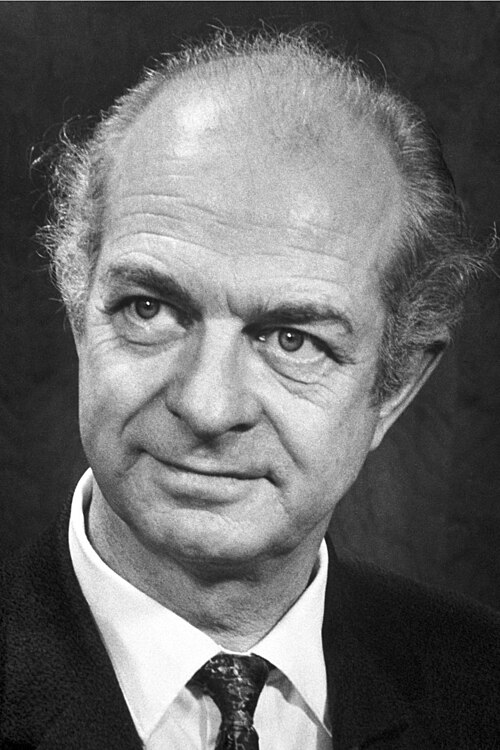
\includegraphics[width=0.24\linewidth]{images/book2/pauling.jpg}

{\small Linus Pauling (1901--1994).}
\end{omfigure}

\section{Évolution du caractère chimique}

\begin{proposition}[Caractère réducteur et caractère oxydant]\label{prop:b1:periodicity:redox-trend}
Les éléments de faible énergie d'ionisation et de faible
\omterm{def:b1:periodicity:electronegativity}{électronégativité}, à gauche du tableau et en bas de leurs groupes,
perdent facilement des électrons~: ce sont des métaux réducteurs (les
métaux alcalins avant tout). Les éléments de forte \omterm{def:b1:periodicity:electronegativity}{électronégativité} et
de forte \omterm{def:b1:periodicity:electron-affinity}{affinité électronique}, en haut à droite, gagnent facilement des
électrons~: ce sont des non-métaux oxydants (le fluor, l'oxygène et le
chlore avant tout). Les gaz nobles, d'énergie d'ionisation élevée et
sans affinité pour un électron supplémentaire, ne font ni l'un ni
l'autre.
\end{proposition}

\begin{method}[Prévoir une tendance à partir de la position]\label{met:b1:periodicity:predict}
Pour comparer deux éléments vis-à-vis d'une propriété liée à l'emprise
du noyau sur les \omterm{def:b1:quantum-numbers:configuration}{électrons de valence} (rayon, $E_i$, $E_{ea}$, $\chi$)~:
\begin{enumerate}
  \item s'ils sont dans le même groupe, celui qui est plus bas a le plus
        grand $n$~: rayon plus grand, $E_i$ et $\chi$ plus faibles~;
  \item s'ils sont dans la même \omterm{def:b1:periodicity:table}{période}, celui qui est plus à droite a la
        plus grande $Z^{*}$~: rayon plus petit, $E_i$ et $\chi$ plus
        grandes~;
  \item sinon, comparer chacun à l'élément situé à l'intersection de sa
        ligne et de la colonne de l'autre~;
  \item vérifier les effets de \omterm{def:b1:quantum-numbers:orbital}{sous-couche} (début d'une \omterm{def:b1:quantum-numbers:orbital}{sous-couche} p,
        premier électron p apparié) avant de conclure sur les énergies
        d'ionisation.
\end{enumerate}
\end{method}

\begin{example}[Le lithium dans une batterie]\label{ex:b1:periodicity:lithium}
Le lithium a la plus faible \omterm{def:b1:periodicity:electronegativity}{électronégativité} de la \omterm{def:b1:periodicity:table}{période} 2 et perd
facilement son électron 2s, tout en étant le plus léger des métaux~: il
transporte plus de charge échangeable par gramme que tout autre élément,
et c'est pourquoi il alimente les batteries rechargeables. Son \omterm{def:b1:periodicity:ionisation-energy}{énergie de
première ionisation}, \qty{5.39}{eV}, est supérieure à celle du sodium
(5.14) ou du potassium (4.34), et pourtant, dans l'eau, c'est le plus
réducteur des métaux alcalins~: ce paradoxe s'explique par la forte
hydratation du petit ion \ce{Li+} (\cref{ch:b1:nernst}).
% ledger: ie:Li, ie:Na, ie:K
\end{example}

\section{Exercices}

\begin{exercise}[$\star$]\label{exo:b1:periodicity:1}
Donner la \omterm{def:b1:periodicity:table}{période}, le groupe et le \omterm{def:b1:periodicity:table}{bloc} du calcium, du fer, du sélénium
et de l'iode ($Z = 20, 26, 34, 53$), à partir de leurs configurations.
\end{exercise}

\begin{exercise}[$\star$]\label{exo:b1:periodicity:2}
Dans chaque couple, quelle espèce est la plus grosse, et pourquoi~?
\ce{Na} ou \ce{Cl}~; \ce{Na} ou \ce{Na+}~; \ce{F-} ou \ce{Cl-}~; \ce{Na+} ou \ce{Mg^{2+}}.
\end{exercise}

\begin{exercise}[$\star$]\label{exo:b1:periodicity:3}
Les \omterm{def:b1:periodicity:ionisation-energy}{énergies de première ionisation} de \ce{Na}, \ce{Mg}, \ce{Al}, \ce{P},
\ce{S} et \ce{Ar} valent 5.14, 7.65, 5.99, 10.49, 10.36 et
\qty{15.76}{eV}. Les classer et relever les deux écarts à la tendance
générale.
\end{exercise}

\begin{exercise}[$\star$]\label{exo:b1:periodicity:4}
Définir la \omterm{def:b1:periodicity:polarisability}{polarisabilité} d'une espèce. Lequel est le plus polarisable,
\ce{F-} ou \ce{I-}~? \ce{Na+} ou \ce{Cl-}~? Justifier.
\end{exercise}

\begin{exercise}[$\star\star$]\label{exo:b1:periodicity:5}
Les quatre premières énergies d'ionisation d'un élément de la \omterm{def:b1:periodicity:table}{période} 3
valent 5.99, 18.83, 28.45 et \qty{119.99}{eV}. Calculer les rapports
successifs, identifier l'élément et l'ion qu'il forme.
\end{exercise}

\begin{exercise}[$\star\star$]\label{exo:b1:periodicity:6}
Expliquer pourquoi le chlore a une \omterm{def:b1:periodicity:electron-affinity}{affinité électronique} plus grande que
le fluor, et pourquoi l'azote et le magnésium ne forment aucun anion
gazeux stable.
\end{exercise}

\begin{exercise}[$\star\star$]\label{exo:b1:periodicity:7}
Calculer les \omterm{def:b1:periodicity:electronegativity}{électronégativités} de Mulliken du sodium ($E_{i1} =
\qty{5.14}{eV}$, $E_{ea} = \qty{0.55}{eV}$) et du chlore ($E_{i1} =
\qty{12.97}{eV}$, $E_{ea} = \qty{3.61}{eV}$). Que disent-elles de la
liaison dans \ce{NaCl}~?
\end{exercise}

\begin{exercise}[$\star\star$]\label{exo:b1:periodicity:8}
À l'aide des valeurs de Pauling de l'\cref{ex:b1:periodicity:bonds} et
de $\chi(\ce{F})
= 3.98$, classer les liaisons \ce{H-F}, \ce{C-H}, \ce{Na-Cl}, \ce{C-Cl}
($\chi(\ce{Cl}) = 3.16$) et \ce{O-H}, et donner le signe de la charge
partielle portée par chaque atome.
\end{exercise}

\begin{exercise}[$\star\star$]\label{exo:b1:periodicity:9}
Les \omterm{def:b1:periodicity:ionisation-energy}{énergies de première ionisation} de \ce{Li}, \ce{Na} et \ce{K} valent
5.39, 5.14 et \qty{4.34}{eV}. Expliquer la tendance et prévoir si celle
du rubidium est supérieure ou inférieure à \qty{4.34}{eV}.
\end{exercise}

\begin{exercise}[$\star\star\star$]\label{exo:b1:periodicity:10}
Le zinc ($Z = 30$) a une \omterm{def:b1:periodicity:ionisation-energy}{énergie de première ionisation} de
\qty{9.39}{eV} et le gallium ($Z = 31$) de \qty{6.00}{eV}~; l'arsenic
($Z = 33$) \qty{9.79}{eV} et le sélénium ($Z = 34$) \qty{9.75}{eV}.
Expliquer les deux baisses à l'aide des configurations.
\end{exercise}

\begin{exercise}[$\star\star\star$]\label{exo:b1:periodicity:11}
On donne $D(\ce{H-H}) = \qty{436}{kJ/mol}$, $D(\ce{F-F}) =
\qty{158}{kJ/mol}$, $\chi(\ce{H}) = 2.20$ et $\chi(\ce{F}) = 3.98$, avec
$\qty{1}{eV} = \qty{96.5}{kJ/mol}$. Estimer l'énergie de liaison
$D(\ce{H-F})$ à l'aide de la définition de Pauling. Pourquoi est-elle
tellement plus grande que la moyenne des deux liaisons symétriques~?
\end{exercise}

\begin{exercise}[$\star\star\star$]\label{exo:b1:periodicity:12}
Les \omterm{def:b1:periodicity:electronegativity}{électronégativités} de Pauling sont tabulées pour le krypton (3.00) et
le xénon (2.60), mais pas pour l'hélium, le néon ou l'argon. À l'aide de
la définition de l'échelle, expliquer pourquoi une valeur ne peut être
donnée que pour un élément qui forme des liaisons, et pourquoi ce sont les
gaz nobles les plus lourds qui en forment.
% ledger: en:Kr, en:Xe
\end{exercise}

\section{Problème~: l'arithmétique de Pauling}

\begin{problem}[{Problème du week-end --- un élément inconnu identifié par
ses énergies d'ionisation, une série d'ions au nuage de même taille, deux
échelles d'électronégativité, et le nombre de Pauling pour la liaison H--Cl}]
\label{pb:b1:periodicity:1}
Donnée~: $\qty{1}{eV}$ par particule correspond à \qty{96.485}{kJ/mol}.

\medskip
\noindent\textbf{Partie I --- Un élément inconnu.}
Les quatre premières énergies d'ionisation d'un élément X de la
\omterm{def:b1:periodicity:table}{période} 3 valent 7.65, 15.04, 80.14 et \qty{109.27}{eV}.
\begin{enumerate}
  \item Pourquoi chaque énergie d'ionisation est-elle supérieure à la
        précédente~?
  \item Calculer les rapports $E_{i2}/E_{i1}$, $E_{i3}/E_{i2}$ et
        $E_{i4}/E_{i3}$.
  \item En déduire le groupe de X, puis l'identifier.
  \item Quel ion X forme-t-il dans ses composés~? Donner sa configuration.
  \item X est-il un métal ou un non-métal~? Justifier à partir de sa position.
  \item Pourquoi le troisième électron coûte-t-il tellement plus que le
        deuxième~?
\end{enumerate}

\medskip
\noindent\textbf{Partie II --- Dix électrons.}
Les \omterm{def:b1:periodicity:radius}{rayons ioniques} (six voisins) de \ce{O^{2-}}, \ce{F-}, \ce{Na+},
\ce{Mg^{2+}} et \ce{Al^{3+}} valent 140, 133, 102, 72 et \qty{54}{pm}.
\begin{enumerate}[resume]
  \item Montrer que ces ions ont la même configuration.
  \item Expliquer le classement des rayons.
  \item Lequel des cinq ions est le plus polarisable, et pourquoi~?
  \item Calculer le rapport du plus grand rayon au plus petit.
  \item La longueur de liaison de \ce{Cl2} vaut \qty{198.8}{pm} et le
        rayon de \ce{Cl-} \qty{181}{pm}. Calculer le \omterm{def:b1:periodicity:radius}{rayon covalent} du
        chlore et comparer.
  \item Sans autre donnée, classer \ce{Cl-}, \ce{Na+} et \ce{Mg^{2+}}
        par taille.
\end{enumerate}

\medskip
\noindent\textbf{Partie III --- L'\omterm{def:b1:periodicity:electronegativity}{échelle de Mulliken}.}
\begin{center}
\small
\begin{tabular}{lccccc}
\hline
élément & \ce{F} & \ce{Cl} & \ce{Br} & \ce{O} & \ce{C} \\
\hline
$E_{i1}$ (eV) & 17.42 & 12.97 & 11.81 & 13.62 & 11.26 \\
$E_{ea}$ (eV) & 3.40 & 3.61 & 3.36 & 1.44 & 1.26 \\
$\chi$ de Pauling & 3.98 & 3.16 & 2.96 & 3.44 & 2.55 \\
\hline
\end{tabular}
\end{center}
% ledger: ie:F, ie:Cl, ie:Br, ie:O, ie:C, ea:F, ea:Cl, ea:Br, ea:O, ea:C,
% en:F, en:Cl, en:Br, en:O, en:C
\begin{enumerate}[resume]
  \item Calculer les \omterm{def:b1:periodicity:electronegativity}{électronégativités} de Mulliken des cinq éléments.
  \item Les classer sur chaque échelle. Quel élément est placé
        différemment~?
  \item Calculer le rapport $\chi_{\text{Pauling}}/\chi_M$ pour les trois
        halogènes. Que remarque-t-on~?
  \item Proposer une raison pour laquelle l'oxygène s'écarte de la règle
        des halogènes (examiner son \omterm{def:b1:periodicity:electron-affinity}{affinité électronique}).
  \item Quel atome porte la charge partielle négative dans \ce{HCl}~?
        dans \ce{ClF}~?
  \item Avec les valeurs tabulées ($\chi(\ce{H}) = 2.20$), la liaison
        \ce{H-Cl} est-elle apolaire, covalente polarisée ou ionique~?
\end{enumerate}

\medskip
\noindent\textbf{Partie IV --- Le nombre de Pauling pour H--Cl.}
Les enthalpies standard de formation de \ce{H(g)}, \ce{Cl(g)} et
\ce{HCl(g)} à \qty{298}{K} valent 218.0, 121.3 et \qty{-92.3}{kJ/mol}~;
celles de \ce{H2(g)} et de \ce{Cl2(g)} sont nulles. On prend pour
énergie de liaison d'une molécule l'enthalpie de sa dissociation en atomes.
% ledger: janaf:H, janaf:Cl, janaf:HCl
\begin{enumerate}[resume]
  \item Calculer $D(\ce{H-H})$ à partir de \ce{H2(g) -> 2H(g)}.
  \item Calculer $D(\ce{Cl-Cl})$.
  \item Calculer $D(\ce{H-Cl})$ à partir de \ce{HCl(g) -> H(g) + Cl(g)}.
  \item Calculer l'énergie excédentaire de Pauling $\Delta E$ en kJ/mol,
        et montrer qu'elle est égale à $-\Delta_f H(\ce{HCl})$.
  \item Convertir $\Delta E$ en électronvolts.
  \item Calculer $|\chi(\ce{Cl}) - \chi(\ce{H})|$ et comparer à la
        différence des valeurs tabulées, $3.16 - 2.20$.
\end{enumerate}
\end{problem}
